 \chapter{Introdução}\label{chp:intro}

% colocar o zhang nas referências (CADE?)
A epilepsia é uma doença crônica comum que atinge aproximadamente 50 milhões de pessoas no mundo todo e, além disso, observa-se uma taxa de mortalidade prematura entre duas a três vezes maior em relação em indivíduos de até 5 anos de idade que apresentam a doença. \cite{EPILEP}. Até o diagnóstico completo do paciente, as crises têm manifestações imprevisíveis no comportamento, no controle muscular, na consciência ou na sensibilidade do indivíduo, dificultando muito a percepção de uma crise \cite{OQ_E}.

% citar artigo sobre video eeg
O EEG (eletroencefalograma) é um exame que mede a atividade elétrica do cérebro, denominadas ondas cerebrais. Por meio da colagem de eletrodos na escalpe do paciente, podemos fazer o registro das ondas e coletar informações necessárias para o diagnóstico particular daquele paciente. No entanto, em casos particulares, não basta ter somente as informações coletadas do EEG para a produção do diagnóstico, para isso, pode-se prolongar a sessão para até 6 horas ou então optar pelo vídeo-EEG \cite{VIDEOEEG}.

\begin{figure}[H]
    \centering
    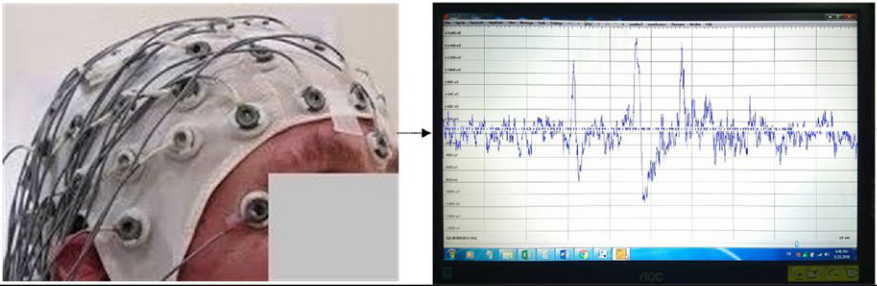
\includegraphics[width=0.7\textwidth]{figuras/Exame_EEG.png}
    \caption{Eletrodos posicionados para o exame EEG e dados obtidos. Fonte: \cite{Siddiqui2020}}
    \label{fig:Exame}
\end{figure}

O vídeo-EEG é uma técnica que consiste em criar uma longa sessão de monitoramento em tempo real, visando detectar uma crise epiléptica com os dados das atividades cerebrais e mudanças de comportamento com o auxílio de câmeras \cite{VIDEOEEG}. Nesses procedimentos a detecção é feita de forma manual, com uma equipe propondo atividades diversas para o paciente e uma outra equipe analisando seu comportamento e seus sinais cerebrais. Porém, esse processo pode apresentar falhas e atrasos da detecção de uma crise, impactando negativamente no tratamento do paciente\cite{VIDEOEEG}.

%e eletrodos são posicionados na superfície da cabeça medindo a flutuação das tensões dada pelas correntes geradas durante as sinapses (correntes iônicas). Nesses procedimentos a detecção da epilepsia é feita de forma manual, com operadores analisando constantemente o paciente e os sinais do EEG do mesmo \cite{}. Entretanto, esse processo pode apresentar falhas ou atrasos durante o vídeo-EEG, como a não percepção de uma crise instantaneamente ou mesmo por completo. Isso é prejudicial para o diagnóstico e retarda o tratamento.

\section{Inspiração na literatura}

A aplicação de métodos em \textit{machine learning} para a realização de objetivos como detecção e predição de crises epilépticas são recorrentes na literatura, como foi apresentado no artigo \textit{''A review of epileptic seizure detection using machine learning classifiers''} \cite{Siddiqui2020}. Esse trabalho presentou sistemas que utilizam aprendizado de máquina para a predição e detecção das crises como auxílio para as sessões de vídeo-EEG. 

A predição consiste em encontrar um momento ''pré-crise'' durante o monitoramento dos sinais do EEG do paciente. Isso permite que a equipe médica receba um alerta prévio para realizar os preparos para o diagnóstico, como inserção de contraste e ressonância magnética. Já na detecção de crises, o modelo objetiva inferir o momento de início da crise, informando o momento exato da disfunção neurológica.

%\section{Objetivo}

%O projeto tem a função de estudar métodos de aprendizado de máquina para o problema de detecção de crises epilépticas. O estudo de diferentes modelos para essa função deve ser abordado, bem como a revisão sobre o estado da arte na literatura.